% Mergen Scope: S21 Gain | 3 dB BW, 2026-11-21
% Preamble: \usepackage{pgfplots} \pgfplotsset{compat=1.18}
\definecolor{msTraceA}{RGB}{86,113,216}
\definecolor{msTraceB}{RGB}{194,73,118}
\definecolor{msTraceC}{RGB}{154,40,46}
\begin{figure}[t]
  \centering
  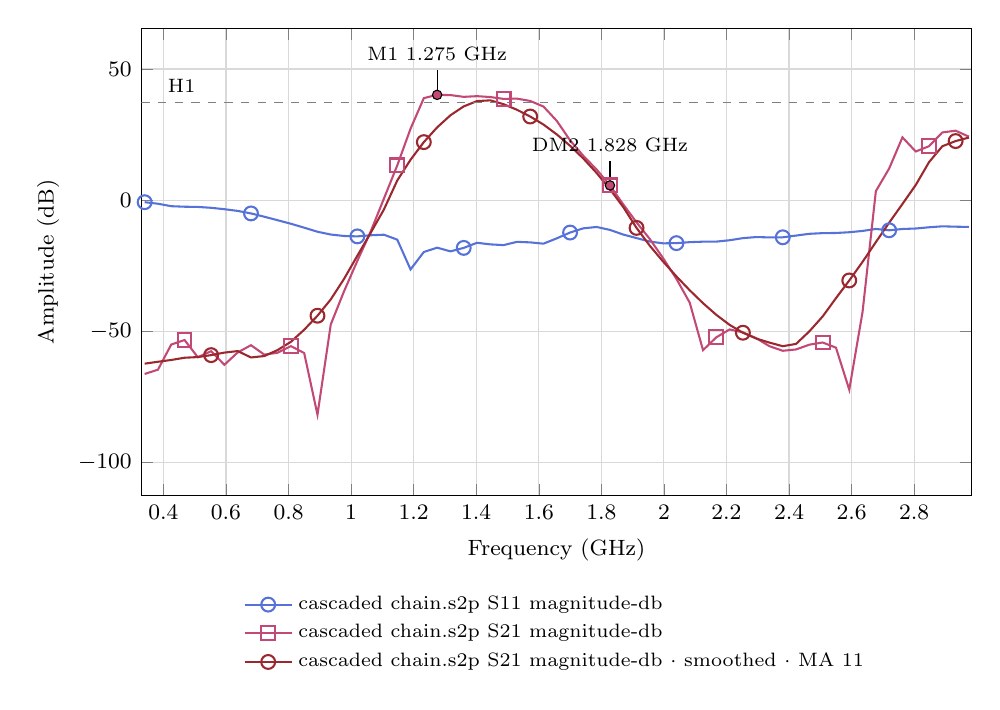
\begin{tikzpicture}
    \begin{axis}[
      width=\columnwidth, height=0.62\columnwidth,
      xmin=0.329601, xmax=2.98368, ymin=-112.648, ymax=65.562,
      xlabel={Frequency (GHz)}, ylabel={Amplitude (dB)},
      grid=major, grid style={gray!30, line width=0.4pt}, axis line style={black},
      tick label style={font=\footnotesize}, label style={font=\footnotesize},
      scaled ticks=false, tick align=inside, clip=true,
      every axis plot/.append style={line width=0.75pt, mark size=2.5pt},
      legend style={at={(0.5,0)}, yshift=-32pt, anchor=north, draw=none, font=\scriptsize, cells={anchor=west}},
      legend columns=1, legend cell align=left,
    ]
      \addplot[color=msTraceA, solid, mark=o, mark repeat=8, mark phase=1, mark options={solid}] coordinates {
        (0.34001,-0.766116) (0.38251,-1.35402) (0.425009,-2.29322) (0.467509,-2.49317) (0.510009,-2.57385) (0.552509,-2.90733)
        (0.595009,-3.44022) (0.637509,-4.0938) (0.680009,-5.05504) (0.722509,-6.31101) (0.765009,-7.6406) (0.807509,-8.98438)
        (0.850009,-10.4874) (0.892509,-12.028) (0.935009,-13.0969) (0.977509,-13.6477) (1.02001,-13.8043) (1.06251,-13.3745)
        (1.10501,-13.1651) (1.14751,-15.0472) (1.19001,-26.4024) (1.23251,-19.7581) (1.27501,-18.1066) (1.31751,-19.5122)
        (1.36001,-18.1891) (1.40251,-16.2427) (1.44501,-16.8533) (1.48751,-17.1326) (1.53001,-15.8891) (1.57251,-16.0893)
        (1.61501,-16.5802) (1.65751,-14.5525) (1.70001,-12.341) (1.74251,-10.7261) (1.78501,-10.2152) (1.82751,-11.3358)
        (1.87001,-13.1074) (1.91251,-14.455) (1.95501,-15.7845) (1.99751,-16.4523) (2.04001,-16.3769) (2.08251,-16.0017)
        (2.12501,-15.82) (2.16751,-15.7942) (2.21001,-15.2748) (2.25251,-14.4691) (2.29501,-14.059) (2.33751,-14.1959)
        (2.38001,-14.1503) (2.42251,-13.493) (2.46501,-12.8226) (2.50751,-12.566) (2.55001,-12.5043) (2.59251,-12.2234)
        (2.63501,-11.7242) (2.67751,-10.9704) (2.72001,-11.4815) (2.76251,-10.9873) (2.80501,-10.8039) (2.84751,-10.3334)
        (2.89001,-9.96881) (2.93251,-10.106) (2.97501,-10.2035)
      };
      \addlegendentry{cascaded chain.s2p S11 magnitude-db}
      \addplot[color=msTraceB, solid, mark=square, mark repeat=8, mark phase=4, mark options={solid}] coordinates {
        (0.34001,-66.2566) (0.38251,-64.6291) (0.425009,-55.0443) (0.467509,-53.3069) (0.510009,-59.8691) (0.552509,-57.5749)
        (0.595009,-62.7512) (0.637509,-58.048) (0.680009,-55.2905) (0.722509,-58.8888) (0.765009,-58.1608) (0.807509,-55.6395)
        (0.850009,-58.2892) (0.892509,-81.7975) (0.935009,-47.3759) (0.977509,-34.7188) (1.02001,-23.1235) (1.06251,-11.9827)
        (1.10501,0.640767) (1.14751,13.2455) (1.19001,27.2484) (1.23251,38.9114) (1.27501,40.1584) (1.31751,40.0691)
        (1.36001,39.398) (1.40251,39.6599) (1.44501,39.321) (1.48751,38.6169) (1.53001,38.7247) (1.57251,37.8368)
        (1.61501,35.7035) (1.65751,30.2365) (1.70001,22.8304) (1.74251,16.8869) (1.78501,11.677) (1.82751,5.63623)
        (1.87001,-1.61142) (1.91251,-8.46536) (1.95501,-14.8307) (1.99751,-22.1334) (2.04001,-30.0068) (2.08251,-39.0807)
        (2.12501,-57.178) (2.16751,-52.2858) (2.21001,-49.2877) (2.25251,-50.3991) (2.29501,-52.6188) (2.33751,-55.6793)
        (2.38001,-57.4232) (2.42251,-56.9095) (2.46501,-55.0852) (2.50751,-54.2583) (2.55001,-56.2301) (2.59251,-72.2562)
        (2.63501,-42.6012) (2.67751,3.43309) (2.72001,12.0818) (2.76251,23.9485) (2.80501,18.5592) (2.84751,20.5759)
        (2.89001,25.8356) (2.93251,26.4948) (2.97501,24.2094)
      };
      \addlegendentry{cascaded chain.s2p S21 magnitude-db}
      \addplot[color=msTraceC, solid, mark=o, mark repeat=8, mark phase=6, mark options={solid}] coordinates {
        (0.34001,-62.332) (0.38251,-61.6087) (0.425009,-60.9252) (0.467509,-60.0732) (0.510009,-59.8147) (0.552509,-59.0746)
        (0.595009,-58.1094) (0.637509,-57.533) (0.680009,-59.9651) (0.722509,-59.4259) (0.765009,-57.1395) (0.807509,-54.0076)
        (0.850009,-49.3923) (0.892509,-44.0569) (0.935009,-37.8264) (0.977509,-29.9957) (1.02001,-21.171) (1.06251,-12.4621)
        (1.10501,-3.52042) (1.14751,7.49735) (1.19001,15.4097) (1.23251,22.1406) (1.27501,27.7533) (1.31751,32.3631)
        (1.36001,35.7446) (1.40251,37.7862) (1.44501,38.0578) (1.48751,36.5959) (1.53001,34.4803) (1.57251,31.8992)
        (1.61501,28.83) (1.65751,25.0781) (1.70001,20.7338) (1.74251,15.875) (1.78501,10.3424) (1.82751,4.1748)
        (1.87001,-2.62377) (1.91251,-10.5705) (1.95501,-17.3993) (1.99751,-23.4152) (2.04001,-29.0584) (2.08251,-34.3543)
        (2.12501,-39.2696) (2.16751,-43.7203) (2.21001,-47.5457) (2.25251,-50.5413) (2.29501,-52.746) (2.33751,-54.305)
        (2.38001,-55.6757) (2.42251,-54.7953) (2.46501,-50.0025) (2.50751,-44.3224) (2.55001,-37.3618) (2.59251,-30.6128)
        (2.63501,-23.522) (2.67751,-15.9997) (2.72001,-8.58336) (2.76251,-1.44993) (2.80501,5.78538) (2.84751,14.4955)
        (2.89001,20.5593) (2.93251,22.5384) (2.97501,23.8698)
      };
      \addlegendentry{cascaded chain.s2p S21 magnitude-db $\cdot$ smoothed $\cdot$ MA 11}
      \draw[gray, dashed, line width=0.5pt] (axis cs:0.329601,37.1584) -- (axis cs:2.98368,37.1584) node[pos=0.02, anchor=south west, font=\scriptsize, text=black] {H1};
      \node[circle, fill=msTraceB, draw=black, inner sep=1.2pt, pin={[font=\scriptsize, pin distance=7pt, pin edge={black, thin}]90:{M1 1.275 GHz}}] at (axis cs:1.27501,40.1584) {};
      \node[circle, fill=msTraceB, draw=black, inner sep=1.2pt, pin={[font=\scriptsize, pin distance=7pt, pin edge={black, thin}]90:{DM2 1.828 GHz}}] at (axis cs:1.82751,5.63623) {};
    \end{axis}
  \end{tikzpicture}
  \caption{S21 Gain \textbar{} 3 dB BW.}
  \label{fig:s21-gain-3-db-bw}
\end{figure}
